\clearpage

\section{Netxpto}

\begin{tcolorbox}	
	\begin{tabular}{p{2.75cm} p{0.2cm} p{10.5cm}} 	
		\textbf{Header File}   &:& netxpto.h\\
                               &:& netxpto\_20180118.h\\
                               &:& netxpto\_20180418.h\\
		\textbf{Source File}   &:& netxpto.cpp \\
                               &:& netxpto\_20180118.cpp \\
                               &:& netxpto\_20180418.cpp \\
	\end{tabular}
\end{tcolorbox}

The netxpto files define and implement the major entities of the simulator.

Namely the signal value possible types
\begin{center}
\begin{tabular}{|c|l|}
    \hline
    Signal Value Type & Data Range\\
    \hline
    BinaryValue         & \{0,1\} \\
    IntegerValue        & $\mathbb{Z}$ \\
    RealValue           & $\mathbb{R}$ \\
    ComplexValue        & $\mathbb{C}$ \\
    ComplexValueXY      & $(\mathbb{C}, \mathbb{C})$ \\
    PhotonValue         & \\
    PhotonValueMP       & \\
    PhotonValueMPXY     & \\
    Message             & \\
    \hline
\end{tabular}
\end{center}


%This block can work in two configurations: with an external clock or without it. In the latter it accepts two input signals one being the clock and the other the signal to be demodulated. In the other configuration there's only one input signal which is the signal.
%
%The output signal is obtained by sampling the input signal with a predetermined samplig rate provided either internally or by the clock.
%
%\subsection*{Input Parameters}
%
%\begin{table}[h]
%	\centering
%	\begin{tabular}{|c|c|p{60mm}|c|ccp{60mm}}
%		\cline{1-4}
%		\textbf{Parameter} & \textbf{Type} & \textbf{Values} &   \textbf{Default}& \\ \cline{1-4}
%		samplesToSkip & int & any (smaller than the number of samples generated) & $0$ \\ \cline{1-4}
%	\end{tabular}
%	\caption{Sampler input parameters}
%	\label{table:sampler_in_par}
%\end{table}
%
%%\begin{itemize}
%%	\item samplesToSkip\{ 0 \}
%%\end{itemize}
%
%\subsection*{Methods}
%
%Sampler() {}
%\bigbreak
%Sampler(vector$<$Signal *$>$ \&InputSig, vector$<$Signal *$>$ \&OutputSig) :Block(InputSig, OutputSig) {}
%\bigbreak
%void initialize(void)
%\bigbreak
%bool runBlock(void)
%\bigbreak
%void setSamplesToSkip(\texttt{t\_integer} sToSkip)
%
%\subsection*{Functional description}
%
%This block can work with an external clock or without it.
%
%In the case of having an external clock it accepts two input signals. The signal to be demodulate which is complex and a clock signal that is a sequence of Dirac delta functions with a predetermined period that corresponds to the sampling period. The signal and the clock signal are scanned and when the clock has the value of 1.0 the correspondent complex value of the signal is placed in the buffer corresponding to the output signal.
%
%There's a detail worth noting. The electrical filter has an impulse response time length of 16 (in units of symbol period). This means that when modulating a bit the spike in the signal corresponding to that bit will appear 8 units of symbol period later. For this reason there's the need to skip the earlier samples of the signal when demodulating it. That's the purpose of the \textit{samplesToSkip} parameter.
%
%Between the binary source and the current block the signal is filtered twice which means that this effect has to be taken into account twice. Therefore the parameter \textit{samplesToSkip} is given by $2*8*samplesPerSymbol$.
%
%\subsection*{Input Signals}
%
%\subparagraph*{Number:} 1
%
%\subparagraph*{Type:} Electrical real (TimeContinuousAmplitudeContinuousReal)
%
%\subsection*{Output Signals}
%
%\subparagraph*{Number:} 1
%
%\subparagraph*{Type:} Electrical real (TimeDiscreteAmplitudeContinuousReal)
%
%\subsection*{Examples}
%
%\begin{figure}[h]
%	\centering
%	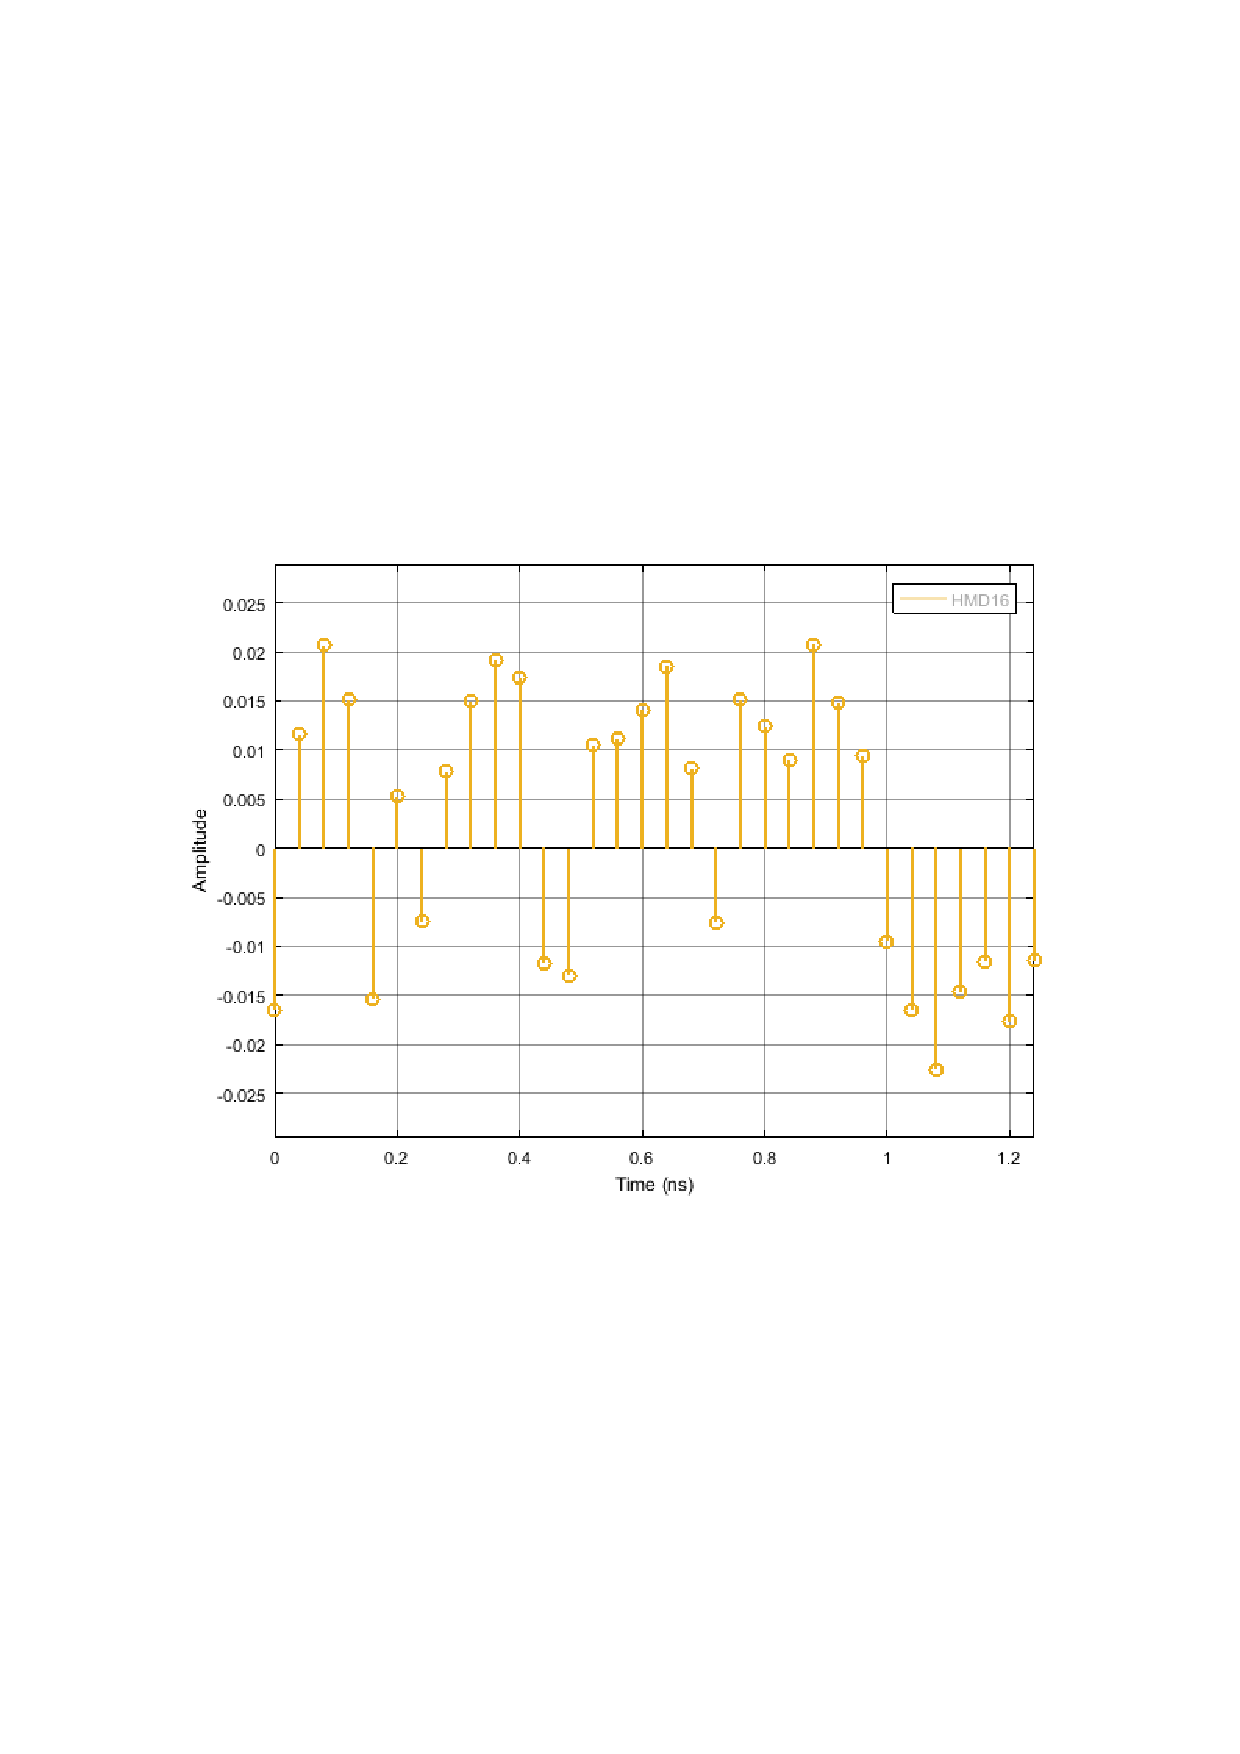
\includegraphics[clip, trim=0.5cm 9cm 0.5cm 9cm, width=\textwidth]{./lib/sampler/figures/MQAM_sampler_output.pdf}
%	\caption{Example of the output signal of the sampler}\label{Sampler_output}
%\end{figure}

\subsection{ Version 20180118}

Adds the type t\_photon\_mp\_xy, to support multi-path photon signals with polarization information.

Changes the signal data type to make private its data structure, only allowing its access through appropriate methods.

\subsection{ Version 20180418}

Adds the possibility to include the parameters from an external file.

\subsection*{Sugestions for future improvement}
